\documentclass{article}
\usepackage[utf8]{inputenc}
\usepackage[includeheadfoot, margin=1em,headheight=2em]{geometry}
\usepackage{titling}
\geometry{a4paper, left=2cm, right=2cm, top=2cm, bottom=2cm}
\usepackage{graphicx}
\usepackage{enumitem}
\usepackage{array}
\usepackage[italian]{babel}
\newcolumntype{P}[1]{>{\centering\arraybackslash}p{#1}}
\renewcommand{\arraystretch}{1.5} % Default value: 1
\setlength{\droptitle}{-6em}

%font
\usepackage[defaultfam,tabular,lining]{montserrat}
\usepackage[T1]{fontenc}
\renewcommand*\oldstylenums[1]{{\fontfamily{Montserrat-TOsF}\selectfont #1}}

%custom bold 
\usepackage[outline]{contour}
\usepackage{xcolor}
\newcommand{\custombold}{\contour{black}}

%table colors
\usepackage{color, colortbl}
\definecolor{Blue}{rgb}{0.51,0.68,0.79}
\definecolor{LightBlue}{rgb}{0.82,0.87,0.90}
\definecolor{LighterBlue}{rgb}{0.93,0.95,0.96}

%Header
\usepackage{fancyhdr, xcolor}
\pagestyle{fancy}
\let\oldheadrule\headrule% Copy \headrule into \oldheadrule
\renewcommand{\headrule}{\color{Blue}\oldheadrule}% Add colour to \headrule
\renewcommand{\headrulewidth}{0.2em}
\fancyhead[L]{Analisi dei reuiqisiti}
\fancyhead[C]{}
\fancyhead[R]{}


\title{\Huge{\textbf{Analisi dei requisiti}}\vspace{-1em}}

\author{CyberSorcerers Team}
\date{}
\begin{document}
\maketitle

\vspace{-3em}
\begin{figure}[h]
  \centering
  
\includegraphics[width=6cm, height=6cm]{logo rotondo.png}
  \label{fig:immagine}
\end{figure}

\vspace{6em}
\large{

\begin{center}
    \begin{tabular}{l c c}
        \rowcolor{Blue} 
        Informazioni sul documento & &\\ [1 ex]
        \rowcolor{LighterBlue}
        Redattori: &Samuele Vigonotto  &Nicola Lazzarin \\ [1 ex]
        \rowcolor{LightBlue}
        Verificatore:  &  &  \\ [1 ex]
        \rowcolor{LighterBlue}
        Destinatari: & Prf. Tullio Vardanega & Prf. Riccardo Cardin\\ [1 ex]


    \end{tabular}
\end{center}}
\newpage
\custombold{Registro dei Cambiamenti - Changelog}

\begin{center}
\begin{tabular}{P{5em} P{5em} P{8em} P{8em} P{10em}} 
  \rowcolor{Blue}
    \custombold{Versione} & \custombold{Data} & \custombold{Autore} &
    \custombold{ Verificatore} & \custombold{Dettaglio}\\
    \rowcolor{LighterBlue}
     0.0.1& 03/12/2023 & Vignotto Samuele & Lazzarin Nicola & Prima stesura dei casi d'uso e dell'analisi dei requisiti.\\
    \rowcolor{LightBlue}
    0.0.1& 09/12/2023 & Caniato Sabrina  & Vignotto Samuele & Definizione struttura del documento e scheletro delle sezioni. Scrittura introduzione ed obiettivi delle diverse sezioni.\\ 
     & &  &  &\\ 
\end{tabular}
\end{center}
\newpage

\section*{Introduzione}

\subsection*{Scopo del documento}

Questo documento ha lo scopo di fornire una descrizione approfondita del prodotto, analizzando nel dettaglio i requisiti, ottenuti tramite incontri con l'azienda e analisi del capitolato. Quest'analisi si concretizza con l'individuazione di casi d'uso, punto centrale di questo documento.


\subsection*{Scopo del prodotto}
L'azienda proponente ha richiesto la creazione di una web app che, tramite l'uso di IA (in questo caso ChatGPT4 e Bedrock) è in grado di creare epic user stories a partire dalle richieste del cliente e confrontarle con il codice sviluppato in modo da informare il cliente dello stato di avanzamento dello sviluppo del prodotto. Inoltre deve essere possibile, sia per il Project Manager, sia per il cliente rilasciare dei feedback (nel primo caso riguardanti l'adeguatezza delle stories,nel secondo caso riguardanti il prodotto finale) al fine di migliorare l'IA. È inoltre richiesta un' analisi comparativa tra le due IA utilizzate e lo sviluppo di un plugin utile agli sviluppatori e al Project Manager.

\subsection*{Glossario}
Alcuni termini presenti nel documento potrebbero essere ambigui, pertanto verranno inseriti nel Glossario v.1.0.0. La loro presenza all'interno di esso sarà indicata tramite una G maiuscola a pedice.

\section*{Casi d'uso}
\subsection*{Scopo}
Lo scopo di questa sezione è raccogliere tutti i casi d'uso individuati, facendo riferimento alle funzionalità individuate durante la sessione di design thinking fatta in collaborazione con l'azienda.

\subsection*{Attori}
Come si è evidenziato durante la sessione di design thinking con i proponenti la web app avrà necessità di tre diverse interfacce per essere usata adeguatamente da tutte le tipologie di attori: clienti, sviluppatori e Project Manager. L'IA (ChatGPT o Bedrock) non viene considerata attore in quanto è parte integrante del sistema. Inoltre è necessario lo sviluppo di un plugin accessibile solamente a agli sviluppatori e al Project Manager.

\newpage
\begin{figure}[h]
    \centering
    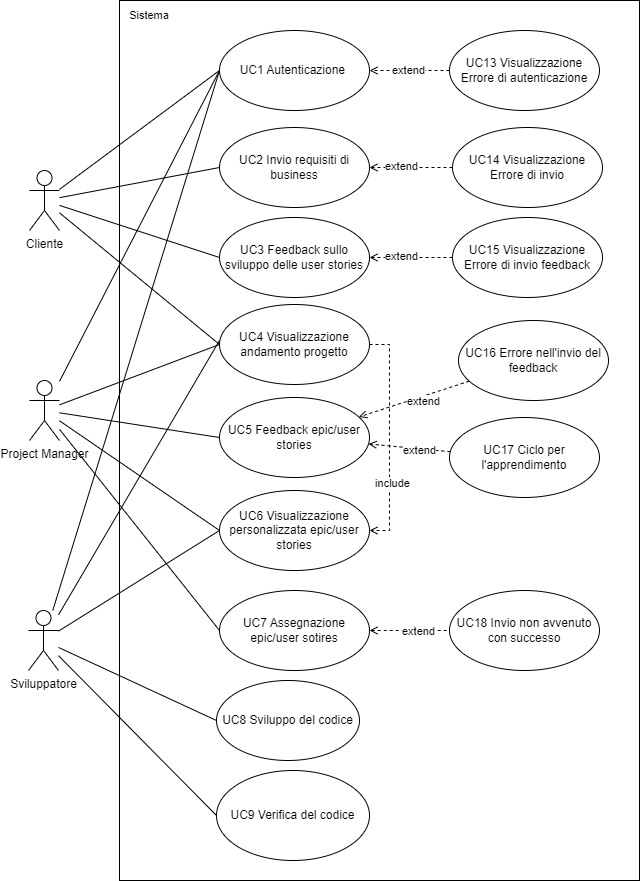
\includegraphics[height = 0.75\textheight]{./imgUML/UML.png}
    \label{fig:immagine}
\end{figure}
\newpage
\section{UC1-Autenticazione}
    \begin{figure}[h]
      \centering
      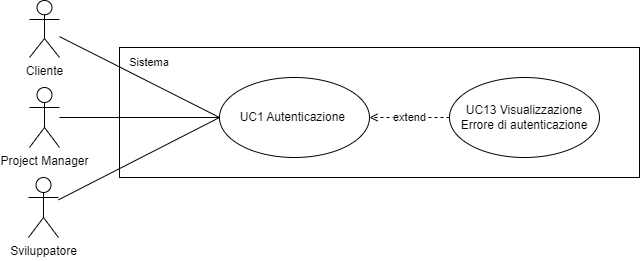
\includegraphics{./imgUML/UC1.png}
      \label{fig:immagine}
    \end{figure} 
    
     \subsection*{Main actor}
         \begin{itemize}
             \item Cliente;
         \end{itemize}
     \subsection*{Preconditions} 
        \begin{itemize}
            \item Essere registrati nel sistema con i propri permessi
        \end{itemize}
               
    \subsection*{Postconitions}
        \begin{itemize}
            \item Utente riconosciuto dal sistema;
        \end{itemize}
    \subsection*{Main scenario}
        \begin{figure}[h]
            \centering
            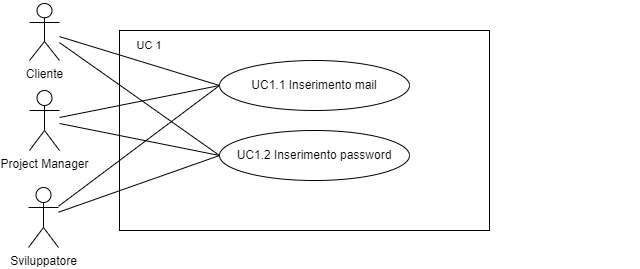
\includegraphics{./imgUML/UC1-zoom.png}
            \label{fig:immagine}
        \end{figure}
            
        \begin{itemize}
            \item Compilazione campo mail [UC1.1.1];
            \item Compilazione campo password [UC1.1.2];
            \item Verifica della correttezza delle credenziali da parte del sistema [UC1.1.3];
            \item Utente riconosciuto [UC1.1.4];
        \end{itemize}
            
        \subsection*{Alternative scenario}
            \begin{itemize}
                \item Compilazione campo mail;
                \item Compilazione campo password;
                \item Verifica della correttezza delle credenziali da parte del sistema;
                \item Warning credenziali non valide [UC13];
            \end{itemize}
    
\section{UC2-Invio requisiti di business}
    \begin{figure}[h]
      \centering
      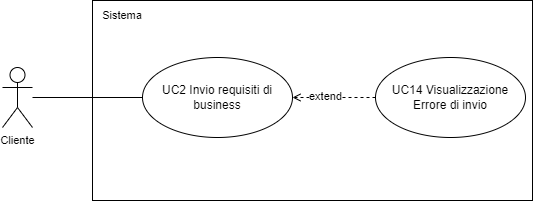
\includegraphics{./imgUML/UC2.png}
      \label{fig:immagine}
    \end{figure}
     \subsection*{Main actor}
     \begin{itemize}
         \item Cliente;
     \end{itemize}
     \subsection*{Preconditions} 
     \begin{itemize}
         \item Essere riconosciuti dal sistema come Cliente;
     \end{itemize}
     \subsection*{Postconitions} 
        \begin{itemize}
            \item Invio requisiti di business al sistema;
        \end{itemize}
     \subsection*{Main scenario}
         \begin{figure}[h]
            \centering
            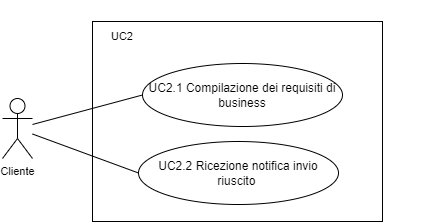
\includegraphics{./imgUML/UC2-zoom.png}
            \label{fig:immagine}
        \end{figure}
        \begin{itemize}
            \item Cliente compila requisiti di business [UC2.1.1];
            \item Cliente invia requisiti di business [UC2.1.2];
            \item Cliente riceve notifica di invio riuscito [UC2.1.3];
        \end{itemize}
     \subsection*{Alternative scenario}
        \begin{itemize}
            \item Cliente compila requisiti di business;
            \item Cliente invia requisiti di business;
            \item Cliente riceve notifica di invio non riuscito [UC14];
        \end{itemize}

\section{UC3-Feedback cliente sullo sviluppo user stories}
    \begin{figure}[h]
      \centering
      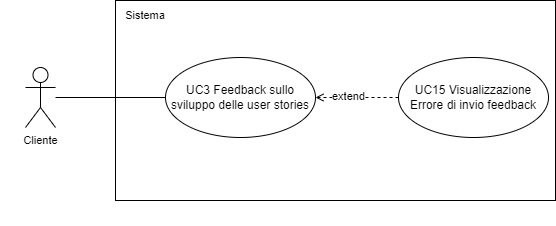
\includegraphics{./imgUML/UC3.png}
      \label{fig:immagine}
    \end{figure}
    
    \subsection*{Main actor}
    \begin{itemize}
        \item Cliente;
    \end{itemize}
    
    \subsection*{Preconditions}
    \begin{itemize}
        \item Essere riconosciuti dal sistema come Cliente;
        \item Presenza di almeno una user story o epic story;
        \item Epic stories completata;
    \end{itemize}
    
    \subsection*{Postconditions}
    \begin{itemize}
        \item Epic/user stories completato;
        \item Feedback per epic/user stories ricevuto dal sistema; 
    \end{itemize}
    
    \subsection*{Main scenario}
        \begin{figure}[h]
            \centering
            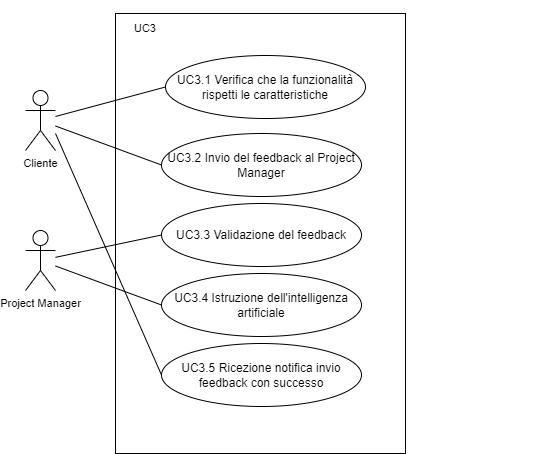
\includegraphics{./imgUML/UC3-zoom.png}
            \label{fig:immagine}
        \end{figure}
        \begin{itemize}
            \item Cliente verifica che la funzionalità sviluppata sia conforme alle sue aspettattive [UC3.1];
            \item Cliente invia il feedback al Project Manager [UC3.2];
            \item Project Manager valida il feedback inviato [UC3.3];
            \item Project Manager istruisce l'intelligenza artificiale [UC3.4];
            \item Cliente riceve notifica di invio feedback con successo [UC3.5];
        \end{itemize}
        
    \subsection*{Alternative scenario}
    \begin{itemize}
        \item Cliente verifica che la funzionalità sviluppata sia conforme alle sue aspettattive;
        \item Cliente invia il feedback al Project Manager;
        \item La notifica non arriva al Project Manager;
        \item Cliente riceve notifica di invio feedback non riuscito [UC15];
    \end{itemize}
      
\section{UC4-Visualizzazione andamento progetto}
    \begin{figure}[h]
      \centering
      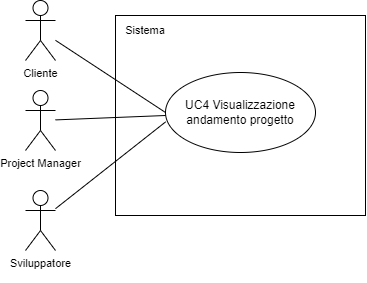
\includegraphics{./imgUML/UC4.png}
      \label{fig:immagine}
    \end{figure}
    
    \subsection*{Main actor}
        \begin{itemize}
            \item Cliente;
            \item Sviluppatore;
            \item Project Manager;
        \end{itemize}
        
    \subsection*{Preconditions}
        \begin{itemize}
            \item Essere riconosciuti dal sistema con i propri privilegi;
            \item Cliente ha inviato con successo i requisiti di business al sistema;
            \item Requisiti di business sono stati elaborati dal sistema;
            \item Project Manager ha accettato le epic/user stories generate dal sistema;
            \item Project Manager ha assegnato le epic/user stories agli Sviluppatori;
        \end{itemize}
        
    \subsection*{Postconitions}
        \begin{itemize}
            \item Presa visione dell'andamento del progetto;
        \end{itemize}
        
    \subsection*{Main scenario}
        \begin{figure}[h]
          \centering
          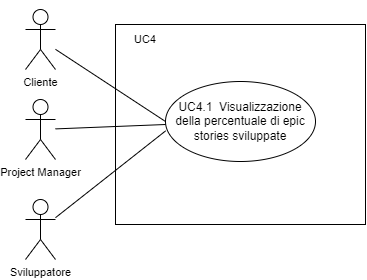
\includegraphics{./imgUML/UC4-zoom.png}
          \label{fig:immagine}
        \end{figure}
        
        \begin{itemize}
            \item Visualizzazione della percentuale rapprensentante il quantitativo di epic/user stories sviluppate [UC4.1];
        \end{itemize}
        

\section{UC5-Feedback epic/user sotries Project Manager}
    \begin{figure}[h]
      \centering
      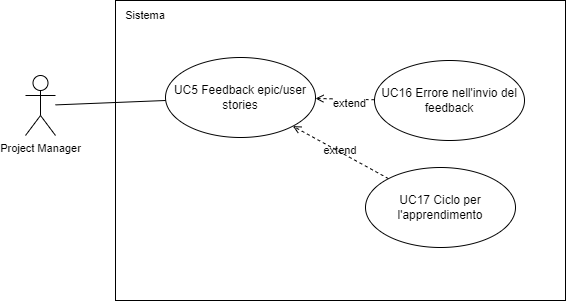
\includegraphics{./imgUML/UC5.png}
      \label{fig:immagine}
    \end{figure}
%con feedback si intende un effetto di reazione prodotto da un messaggio su chi lo ha emesso
    \subsection*{Main actor}
    \begin{itemize}
        \item Project Manager;
    \end{itemize}
    
    \subsection*{Preconditions}
        \begin{itemize}
            \item Essere riconosciuti dal sistema come Project Manager;
            \item Cliente ha inviato con successo i requisiti di businessa al sistema;
            \item Requisiti di business sono stati elaborati dal sistema;
        \end{itemize}
        
    \subsection*{Postconitions}
        \begin{itemize}
            \item Feedback per epic/user stories ricevuto dal sistema;
            \item Il sistema ha generato epic/user sotries corrette, con corrispettivo tag;
        \end{itemize}
        
    \subsection*{Main scenario}
        \begin{figure}[h]
          \centering
          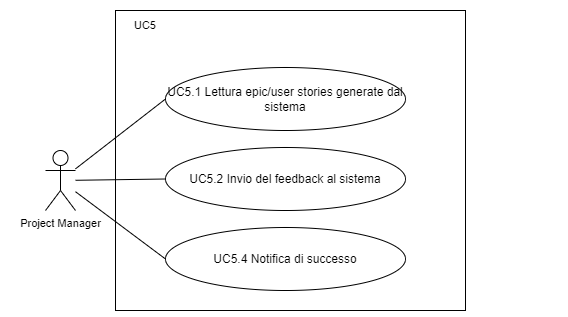
\includegraphics{./imgUML/UC5-zoom-1.png}
          \label{fig:immagine}
        \end{figure}

        \begin{itemize}
            \item Project Manager legge epic/user stories generate dal sistema [UC5.1];
            \item Project Manager invia il feedback al sistema [UC5.2];
            \item Il sistema modifica quanto richiesto dal Project Manager [UC5.3];
            \item Project Manager riceve notifica di invio feedback con successo [UC5.4];
        \end{itemize}
        
    \subsection*{Alternative scenario}
        
        \begin{itemize}
            \item Project Manager legge epic/user stories generate dal sistema [UC16.1];
            \item Project Manager seleziona tipo di feeedback per ogni epic/user story [UC16.2];
            \item Project Manager riceve warning invio feedback non riuscito [UC16.3];
        \end{itemize}
        
    \subsection*{Alternative scenario}      
        \begin{itemize}
            \item Project Manager legge epic/user stories generate dal sistema [UC17.1];
            \item Project Manager invia il feedback al sistema [UC17.2];
            \item Il sistema invia la modifica quanto richiesto dal Project Manager [UC17.3];
            \item Project Manager invia il feedback al sistema [UC17.4];
            \item Project Manager riceve notifica di invio feedback con successo [UC17];        
        \end{itemize}

\section{UC6-Visualizzazione personalizzata epic/user stories}
    \begin{figure}[h]
      \centering
      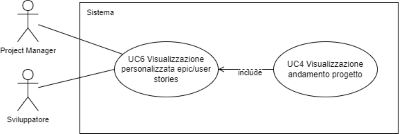
\includegraphics{./imgUML/UC6.png}
      \label{fig:immagine}
    \end{figure}
    
    \subsection*{Main actor}
        \begin{itemize}
            \item Project Manager;
            \item  Sviluppatore;
        \end{itemize}
        
    \subsection*{Preconditions}
        \begin{itemize}
            \item Essere riconosciuti dal sistema con i propri permessi;
            \item Cliente ha inviato con successo i requisiti di businessa al sistema;
            \item requisiti di business sono stati elaborati dal sistema;
            \item Project Manager ha accettato le epic/user stories generate dal sistema;
            \item Project Manager ha assegnato le epic/user stories agli Sviluppatori;
        \end{itemize}
        
    \subsection*{Postconitions}
    \begin{itemize}
        \item Project Manager ha preso visione dell'andamento del progetto;
    \end{itemize}
    
    \subsection*{Main scenario}
        \begin{itemize}
            \item Project Manager visualizza la lista delle epis/user stories assegnate;
        \end{itemize}
        
    \subsection*{Inclusione}
        \begin{itemize}
            \item Visualizzazione andamento progetto [UC4];
        \end{itemize}

\section{UC7-Assegnazione epic/user stories}
    \begin{figure}[h]
      \centering
      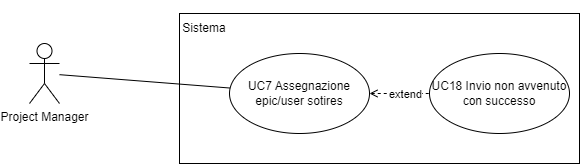
\includegraphics{./imgUML/UC7.png}
      \label{fig:immagine}
    \end{figure}

    \subsection*{Main actor}
    \begin{itemize}
        \item Project Manager;
    \end{itemize}
    
    \subsection*{Secondary actor}
    \begin{itemize}
        \item Sviluppatore;
    \end{itemize}
    
    \subsection*{Preconditions}
        \begin{itemize}
            \item Essere riconosciuto dal sistema come Project Manager;
            \item Le epic/user stories che si vogliono assegnare devono avere feedback positivo;
        \end{itemize}
        
    \subsection*{Postconditions}
        \begin{itemize}
            \item Una o più epic/user story con feedback positivo è stata assegnata ad uno o più Sviluppatori;
        \end{itemize}
    
    \subsection*{Main scenario}
        \begin{figure}[h]
          \centering
          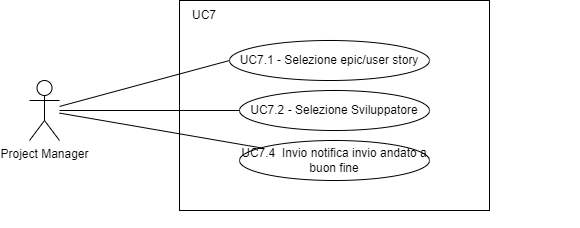
\includegraphics{./imgUML/UC7-zoom.png}
          \label{fig:immagine}
        \end{figure}
        
        \begin{itemize}
            \item Project Manager seleziona epic/user story da assegnare;
            \item Project Manager seleziona lo Sviluppatore a cui assegnare la epic/user story selezionata;
            \item Project Manager conferma selezione;
            \item Project Manager riceve notifica di invio andato a buon fine;
            \item Sviluppatore riceve epic/user story assegnata;
        \end{itemize}
        
    \subsection*{Alternative scenario}
        \begin{itemize}
            \item Project Manager seleziona epic/user story da assegnare;
            \item Project Manager seleziona lo Sviluppatore a cui assegnare la epic/user story selezionata;
            \item Project Manager conferma selezione;
            \item Project Manager riceve warning di invio non riuscito;
        \end{itemize}    

\section{UC8-Sviluppo del codice}
    \begin{figure}[h]
      \centering
      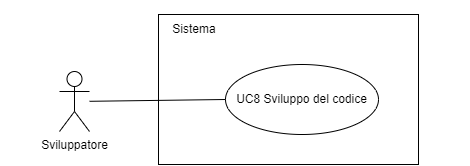
\includegraphics{./imgUML/UC8.png}
      \label{fig:immagine}
    \end{figure}
    
    \subsection*{Main actor}
        \begin{itemize}
            \item Sviluppatore;
        \end{itemize}
    
    \subsection*{Preconditions}
        \begin{itemize}
            \item Essere riconosciuti dal sistema come Sviluppatore;
        \end{itemize}
        
    \subsection*{Postconditions} 
        \begin{itemize}
            \item Il codice svipuppato e pronto per il testing;
            \item Il codice è correttamente taggato;  
        \end{itemize}
    
    \subsection*{Main scenario}
        \begin{figure}[h]
          \centering
          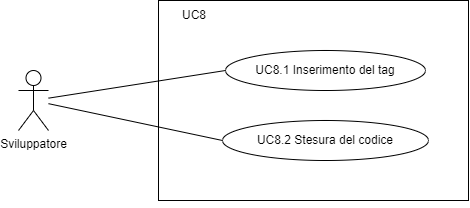
\includegraphics{./imgUML/UC8-zoom.png}
          \label{fig:immagine}
        \end{figure}
        
        \begin{itemize}
            \item Sviluppatore inserisce il tag di riferimento alla user story;
            \item Sviluppatore scrive del codice;
        \end{itemize}

\section{UC9-Verifica codice da parte dell'AI}
    \begin{figure}[h]
      \centering
      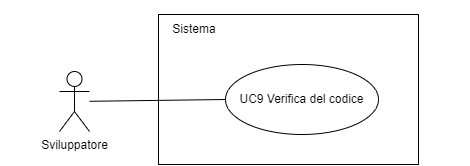
\includegraphics{./imgUML/UC9.png}
      \label{fig:immagine}
    \end{figure}
    
    \subsection*{Main actor}
        \begin{itemize}
            \item Sviluppatore;
        \end{itemize}
        
    \subsection*{Preconditions}
        \begin{itemize}
            \item Essere riconosciuti dal sistema come sviluppatore;
            \item Cliente ha inviato requisiti di business;
            \item Project Manager ha accettato epic/user stories;
            \item Project Manager ha assegnato epic/user stories;
            \item Sviluppatore ha sviluppato codice e test riguardante una o più user story;
            \item Sviluppatore ha taggato correttamente il codice;
        \end{itemize}
        
    \subsection*{Postconditions}
        \begin{itemize}
            \item Sviluppatore riceve feedback da parte del sistema riguardante il codice inviato;
        \end{itemize}
    
    \subsection*{Main scenario}
        \begin{figure}[h]
          \centering
          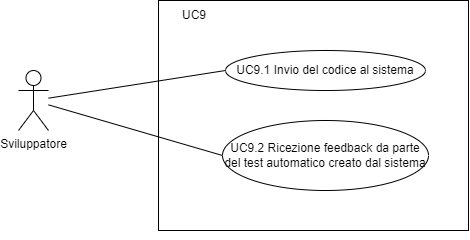
\includegraphics{./imgUML/UC9-zoom.png}
          \label{fig:immagine}
        \end{figure}
        
        \begin{itemize}
            \item Sviluppatore invia codice per la verifica;
            \item Sviluppatore riceve notifica di invio andato a buon fine;
            \item Il sistema crea codice di testing riguardante la user story taggata;
            \item Sviluppatore riceve feedback dal sistema riguardante il codice inviato;
        \end{itemize}
        
    \subsection*{Alternative scenario}
        \begin{itemize}
            \item Sviluppatore invia codice per la verifica;
            \item Sviluppatore riceve warning di invio non riuscito;
        \end{itemize}

\newpage
\section{Requisiti}
\subsection{Requisiti funzionali}
\begin{center}
    \begin{tabular}{|p{3cm}|p{6cm}|p{3,5cm}|p{3cm}|}
    \rowcolor{Blue} 
\hline
Classificazione & Descrizione & Indirizzato a&Codice  \\ 
\rowcolor{LightBlue}
\hline
Obbligatorio & Accesso a web app tramite login composto da email e password & Sviluppatore, Cliente, Project Manager & UC1, UC5, UC9 \\ 
\rowcolor{LighterBlue}
\hline
Obbligatorio & Scrittura di richieste di buisness tramite box testuale da web app & Cliente & UC2\\ 
\rowcolor{LightBlue}
\hline
Obbligatorio & Invio delle richieste di buisness da web app & Cliente & UC2\\
\hline
\rowcolor{LighterBlue}

Obbligatorio & Visualizzazione andamento sviluppo richieste tramite barra di completamento basata sulla percentuale di user stories completate & Cliente, Project Manager & UC4, UC7\\
\rowcolor{LightBlue}
\hline
Obbligatorio & Approvazione o rifiuto del risultato relativo all'implementazione di una user story & Cliente & UC3, UC3.1, UC3.2\\
\hline
\rowcolor{LighterBlue}

Desiderabile & Ricezione notifiche quando user story completata & Cliente & UC4\\
\hline
\rowcolor{LightBlue}
\hline
Obbligatorio & Funzionalità di tag nel plugin  & Sviluppatore & UC10\\
\hline
\rowcolor{LighterBlue}

Obbligatorio & Lista di user stories assegnate da Project Manager sia su web app che su plugin & Sviluppatore & UC12\\
\hline
\rowcolor{LightBlue}

Desiderabile & Ricezione notifica su web app quando nuova users story è assegnata dal Project Manager& Sviluppatore & UC12\\
\hline
\rowcolor{LighterBlue}
Obbligatorio & Invio del codice sviluppato a IA per richiesta verifica& Sviluppatore & UC11\\

\hline
\rowcolor{LightBlue}

Obbligatorio & Visualizzazione users stories generate da IA  & Project Manager & UC7\\
\hline



\end{tabular}

    \begin{tabular}{|p{3cm}|p{6cm}|p{3,5cm}|p{3cm}|}
    \rowcolor{Blue} 
\hline
Classificazione & Descrizione & Indirizzato a&Casi d'uso  \\ 
\rowcolor{LightBlue}
\hline
Obbligatorio & Invio di feedback sulle user stories generate all'IA& Project Manager&UC6, UC6.1, UC6.2, UC6.3\\
\hline
\rowcolor{LighterBlue}

Obbligatorio & Suddivisione delle user stories troppo grandi  & Project Manager& UC6.3\\
\hline
\rowcolor{LightBlue}

Obbligatorio & Assegnazione user stories agli sviluppatori& Project Manager& UC8\\
\hline
\rowcolor{LighterBlue}

Desiderabile & Ricezione notifiche quando user story viene generata in seguito a richiesta del cliente & Project Manager & UC7\\
\hline
\rowcolor{LightBlue}

Obbligatorio & Invio richiesta di modifiche realtive a user stories a IA prima di approvazione& Project Manager& UC6.2, UC6.3\\
\hline
\rowcolor{LighterBlue}

Obbligatorio & Visualizzasione andamento epic/user stories assegnate& Sviluppatore& UC12\\
\hline
\end{tabular}
\end{center}
\end{document}